\documentclass{article}
\usepackage[utf8]{inputenc}

% Essential packages for article format
\usepackage{amsmath, amssymb, amsfonts}
\usepackage{bm}
\usepackage{graphicx}
\usepackage{xcolor}
\usepackage{tcolorbox}
\usepackage[bookmarks=false]{hyperref}
\usepackage{url}
\usepackage{booktabs}
\usepackage{array}
\usepackage{multirow}
\usepackage{enumitem}
\usepackage{tikz}
\usetikzlibrary{arrows.meta, positioning, shapes.geometric}

% Additional packages for a nice tutorial format
\usepackage[margin=1in]{geometry}
\usepackage{fancyhdr}
\usepackage{titlesec}

% Header and footer setup
\pagestyle{fancy}
\fancyhf{}
\rhead{Tutorial: Linear Regression}
\lhead{ES335 - Machine Learning}
\rfoot{Page \thepage}

% Title formatting
\titleformat{\section}{\Large\bfseries\color{blue!75!black}}{\thesection}{1em}{}
\titleformat{\subsection}{\large\bfseries\color{blue!60!black}}{\thesubsection}{1em}{}

% Load conventions after math packages
\usepackage{../../shared/styles/conventions}

% Define counters for examples and exercises
\newcounter{example}
\setcounter{example}{0}
\newcounter{exercise}
\setcounter{exercise}{0}

\title{\textbf{Tutorial: Linear Regression} \\ \textit{The Foundation of Predictive Modeling}}
\author{ES335 - Machine Learning \\ IIT Gandhinagar}
\date{\today}

\begin{document}

\maketitle

\begin{abstract}
Linear regression is the cornerstone of statistical modeling and machine learning. This comprehensive tutorial covers the mathematical foundations, geometric interpretations, optimization methods, and practical applications of linear regression. From simple univariate models to multivariate regression with regularization, learn how to build, evaluate, and interpret linear models effectively.
\end{abstract}

\tableofcontents
\newpage

\section{Introduction: The Prediction Problem}

Imagine you're a real estate agent trying to predict house prices. You notice that larger houses tend to cost more. How can you quantify this relationship and make predictions for new houses?

\begin{center}
\begin{tikzpicture}[scale=0.8]
    % Scatter plot
    \draw[->] (0,0) -- (8,0) node[right] {House Size (sq ft)};
    \draw[->] (0,0) -- (0,6) node[above] {Price (\$100k)};
    
    % Data points
    \foreach \x/\y in {1/1.2, 1.5/1.8, 2/2.1, 2.5/2.7, 3/3.2, 3.5/3.6, 4/4.1, 4.5/4.5, 5/4.8, 5.5/5.2, 6/5.5, 6.5/5.8} {
        \fill[blue] (\x,\y) circle (2pt);
    }
    
    % Best fit line
    \draw[thick, red] (0.5,0.8) -- (7,6);
    \node[red] at (6,5) {$y = mx + b$};
    
    % Labels
    \node[below] at (4,0) {1500};
    \node[left] at (0,3) {3};
\end{tikzpicture}
\end{center}

Linear regression finds the \textbf{best straight line} through the data that minimizes prediction errors. This simple idea forms the foundation of most machine learning algorithms.

\textbf{Why Linear Regression?}
\begin{itemize}
    \item \textbf{Interpretable}: Coefficients have clear meaning
    \item \textbf{Fast}: Closed-form solution exists
    \item \textbf{Robust}: Well-understood statistical properties
    \item \textbf{Baseline}: Good starting point for any regression problem
    \item \textbf{Foundation}: Basis for many advanced methods
\end{itemize}

\section{Mathematical Foundation}

\subsection{The Linear Model}

For a single feature (simple linear regression):
$$y = \beta_0 + \beta_1 x + \epsilon$$

For multiple features (multiple linear regression):
$$y = \beta_0 + \beta_1 x_1 + \beta_2 x_2 + \ldots + \beta_p x_p + \epsilon$$

In matrix form:
$$\vy = \mX\vbeta + \vepsilon$$

where:
\begin{itemize}
    \item $\vy \in \Real^n$: target vector
    \item $\mX \in \Real^{n \times (p+1)}$: design matrix (includes intercept column)
    \item $\vbeta \in \Real^{p+1}$: parameter vector
    \item $\vepsilon \in \Real^n$: error vector
\end{itemize}

\begin{tcolorbox}[colback=blue!5!white,colframe=blue!75!black,title=Example \stepcounter{example}\#\theexample: Matrix Representation]

For 3 houses with features [size, bedrooms]:

$$\mX = \begin{bmatrix} 
1 & 1500 & 3 \\
1 & 2000 & 4 \\
1 & 1200 & 2
\end{bmatrix}, \quad 
\vy = \begin{bmatrix} 
250000 \\
350000 \\
200000
\end{bmatrix}, \quad
\vbeta = \begin{bmatrix}
\beta_0 \\
\beta_1 \\
\beta_2
\end{bmatrix}$$

The model: $\text{Price} = \beta_0 + \beta_1 \times \text{Size} + \beta_2 \times \text{Bedrooms}$
\end{tcolorbox}

\subsection{Least Squares Estimation}

We find parameters $\vbeta$ that minimize the \textbf{sum of squared errors}:

$$\text{SSE}(\vbeta) = \sum_{i=1}^n (y_i - \hat{y}_i)^2 = \sum_{i=1}^n (y_i - \vx_i^T\vbeta)^2$$

In matrix form:
$$\text{SSE}(\vbeta) = \normtwo{\vy - \mX\vbeta}^2 = (\vy - \mX\vbeta)^T(\vy - \mX\vbeta)$$

\textbf{Minimization}:
$$\frac{\partial \text{SSE}}{\partial \vbeta} = -2\mX^T(\vy - \mX\vbeta) = 0$$

This gives the \textbf{normal equations}:
$$\mX^T\mX\vbeta = \mX^T\vy$$

\textbf{Closed-form solution} (when $\mX^T\mX$ is invertible):
$$\hat{\vbeta} = (\mX^T\mX)^{-1}\mX^T\vy$$

\subsection{Geometric Interpretation}

Linear regression projects the target vector $\vy$ onto the column space of $\mX$.

\begin{center}
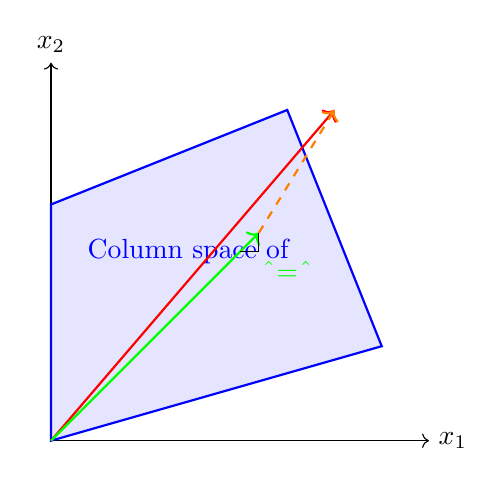
\begin{tikzpicture}[scale=1.2]
    % Coordinate system
    \draw[->] (0,0) -- (4,0) node[right] {$x_1$};
    \draw[->] (0,0) -- (0,4) node[above] {$x_2$};
    
    % Column space (plane)
    \draw[thick, blue, fill=blue!10] (0,0) -- (3.5,1) -- (2.5,3.5) -- (0,2.5) -- cycle;
    \node[blue] at (1.5,2) {Column space of $\mX$};
    
    % True y vector
    \draw[->, thick, red] (0,0) -- (3,3.5);
    \node[red] at (3.3,3.7) {$\vy$};
    
    % Projection
    \draw[->, thick, green] (0,0) -- (2.2,2.2);
    \node[green] at (2.5,1.8) {$\hat{\vy} = \mX\hat{\vbeta}$};
    
    % Error vector
    \draw[->, thick, orange, dashed] (2.2,2.2) -- (3,3.5);
    \node[orange] at (3.2,2.8) {$\vepsilon$};
    
    % Right angle
    \draw (2,2) -- (2.2,2) -- (2.2,2.2);
\end{tikzpicture}
\end{center}

\textbf{Key insight}: $\hat{\vy}$ is the orthogonal projection of $\vy$ onto the column space of $\mX$. The error vector $\vepsilon = \vy - \hat{\vy}$ is orthogonal to this space.

\section{Statistical Properties}

\subsection{Assumptions}

The \textbf{Gauss-Markov assumptions} ensure nice statistical properties:

\begin{enumerate}
    \item \textbf{Linearity}: $E[\vy|\mX] = \mX\vbeta$
    \item \textbf{Independence}: Errors are uncorrelated
    \item \textbf{Homoscedasticity}: $\text{Var}(\epsilon_i) = \sigma^2$ (constant variance)
    \item \textbf{No multicollinearity}: $\mX$ has full column rank
\end{enumerate}

For inference, we also assume:
\begin{enumerate}
    \setcounter{enumi}{4}
    \item \textbf{Normality}: $\epsilon_i \sim \mathcal{N}(0, \sigma^2)$
\end{enumerate}

\subsection{Properties of the OLS Estimator}

Under Gauss-Markov assumptions:

\textbf{Unbiasedness}: $E[\hat{\vbeta}] = \vbeta$

\textbf{Variance}: $\text{Var}(\hat{\vbeta}) = \sigma^2(\mX^T\mX)^{-1}$

\textbf{BLUE}: Best Linear Unbiased Estimator (minimum variance among all linear unbiased estimators)

\textbf{Consistency}: $\hat{\vbeta} \to \vbeta$ as $n \to \infty$

\begin{tcolorbox}[colback=green!5!white,colframe=green!75!black,title=Example \stepcounter{example}\#\theexample: Confidence Intervals]

For coefficient $\beta_j$:
$$\hat{\beta}_j \pm t_{\alpha/2, n-p-1} \times \text{SE}(\hat{\beta}_j)$$

where $\text{SE}(\hat{\beta}_j) = \sqrt{\hat{\sigma}^2 [(\mX^T\mX)^{-1}]_{jj}}$ and $\hat{\sigma}^2 = \frac{\text{SSE}}{n-p-1}$

\textbf{Interpretation}: We're 95\% confident the true coefficient lies in this interval.
\end{tcolorbox}

\section{Model Evaluation}

\subsection{Goodness of Fit}

\textbf{R-squared (Coefficient of Determination)}:
$$R^2 = 1 - \frac{\text{SSE}}{\text{SST}} = 1 - \frac{\sum_i (y_i - \hat{y}_i)^2}{\sum_i (y_i - \bar{y})^2}$$

\textbf{Interpretation}:
\begin{itemize}
    \item $R^2 = 0$: Model explains no variance (as bad as predicting the mean)
    \item $R^2 = 1$: Model explains all variance (perfect fit)
    \item $R^2 = 0.7$: Model explains 70\% of the variance
\end{itemize}

\textbf{Adjusted R-squared} (penalizes for additional features):
$$R^2_{\text{adj}} = 1 - \frac{(1-R^2)(n-1)}{n-p-1}$$

\subsection{Residual Analysis}

\textbf{Residuals}: $e_i = y_i - \hat{y}_i$

\textbf{Diagnostic plots}:
\begin{enumerate}
    \item \textbf{Residuals vs Fitted}: Check linearity and homoscedasticity
    \item \textbf{Q-Q plot}: Check normality of residuals
    \item \textbf{Scale-Location}: Check homoscedasticity
    \item \textbf{Residuals vs Leverage}: Identify influential points
\end{enumerate}

\begin{center}
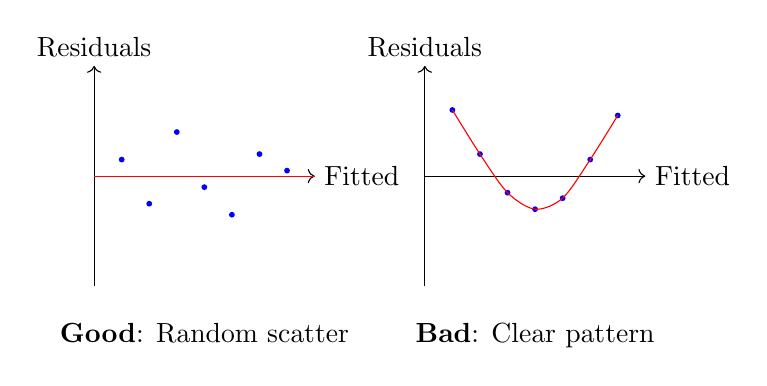
\begin{tikzpicture}[scale=0.7]
    % Good residual plot
    \begin{scope}[xshift=0cm]
        \draw[->] (0,0) -- (4,0) node[right] {Fitted};
        \draw[->] (0,-2) -- (0,2) node[above] {Residuals};
        \foreach \x/\y in {0.5/0.3, 1/-0.5, 1.5/0.8, 2/-0.2, 2.5/-0.7, 3/0.4, 3.5/0.1} {
            \fill[blue] (\x,\y) circle (1.5pt);
        }
        \draw[red] (0,0) -- (4,0);
        \node[below] at (2,-2.5) {\textbf{Good}: Random scatter};
    \end{scope}
    
    % Bad residual plot
    \begin{scope}[xshift=6cm]
        \draw[->] (0,0) -- (4,0) node[right] {Fitted};
        \draw[->] (0,-2) -- (0,2) node[above] {Residuals};
        \foreach \x/\y in {0.5/1.2, 1/0.4, 1.5/-0.3, 2/-0.6, 2.5/-0.4, 3/0.3, 3.5/1.1} {
            \fill[blue] (\x,\y) circle (1.5pt);
        }
        \draw[red, smooth] plot coordinates {(0.5,1.2) (1,0.4) (1.5,-0.3) (2,-0.6) (2.5,-0.4) (3,0.3) (3.5,1.1)};
        \node[below] at (2,-2.5) {\textbf{Bad}: Clear pattern};
    \end{scope}
\end{tikzpicture}
\end{center}

\section{Multiple Linear Regression}

\subsection{Interpretation of Coefficients}

In multiple regression, each coefficient represents the \textbf{partial effect} of that variable, holding all other variables constant.

$$\frac{\partial y}{\partial x_j} = \beta_j$$

\begin{tcolorbox}[colback=orange!5!white,colframe=orange!75!black,title=Example \stepcounter{example}\#\theexample: House Price Model]

$$\text{Price} = 50000 + 100 \times \text{Size} + 15000 \times \text{Bedrooms} + 20000 \times \text{Garage}$$

\textbf{Interpretation}:
\begin{itemize}
    \item \textbf{Baseline}: A house with 0 sq ft, 0 bedrooms, no garage costs \$50,000 (intercept)
    \item \textbf{Size}: Each additional sq ft increases price by \$100, holding bedrooms and garage constant
    \item \textbf{Bedrooms}: Each additional bedroom increases price by \$15,000, holding size and garage constant
    \item \textbf{Garage}: Having a garage increases price by \$20,000, holding size and bedrooms constant
\end{itemize}
\end{tcolorbox}

\subsection{Multicollinearity}

When features are highly correlated, coefficient estimates become unstable.

\textbf{Detection}:
\begin{itemize}
    \item \textbf{Variance Inflation Factor (VIF)}: $\text{VIF}_j = \frac{1}{1-R_j^2}$
    \item \textbf{Condition Number}: $\kappa(\mX^T\mX) = \frac{\lambda_{\max}}{\lambda_{\min}}$
\end{itemize}

\textbf{Rules of thumb}:
\begin{itemize}
    \item VIF $> 5$: Moderate multicollinearity
    \item VIF $> 10$: Severe multicollinearity
    \item Condition number $> 30$: Multicollinearity present
\end{itemize}

\textbf{Solutions}:
\begin{itemize}
    \item Remove highly correlated features
    \item Principal Component Regression (PCR)
    \item Ridge regression (see next section)
\end{itemize}

\section{Advanced Topics}

\subsection{Weighted Least Squares}

When errors have different variances: $\text{Var}(\epsilon_i) = \sigma^2/w_i$

\textbf{Objective function}:
$$\text{WSSE}(\vbeta) = \sum_{i=1}^n w_i(y_i - \vx_i^T\vbeta)^2$$

\textbf{Solution}:
$$\hat{\vbeta} = (\mX^T\mW\mX)^{-1}\mX^T\mW\vy$$

where $\mW = \text{diag}(w_1, \ldots, w_n)$.

\subsection{Polynomial Regression}

Extend linear regression to capture non-linear relationships:

$$y = \beta_0 + \beta_1 x + \beta_2 x^2 + \ldots + \beta_d x^d + \epsilon$$

\textbf{Still linear in parameters}! We can use standard linear regression methods.

\begin{center}
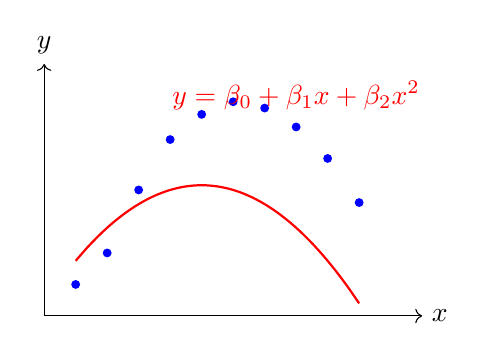
\begin{tikzpicture}[scale=0.8]
    \draw[->] (0,0) -- (6,0) node[right] {$x$};
    \draw[->] (0,0) -- (0,4) node[above] {$y$};
    
    % Data points following a quadratic pattern
    \foreach \x/\y in {0.5/0.5, 1/1, 1.5/2, 2/2.8, 2.5/3.2, 3/3.4, 3.5/3.3, 4/3, 4.5/2.5, 5/1.8} {
        \fill[blue] (\x,\y) circle (2pt);
    }
    
    % Quadratic fit
    \draw[thick, red, smooth] plot[domain=0.5:5] (\x,{0.2 + 1.5*\x - 0.3*\x*\x});
    \node[red] at (4,3.5) {$y = \beta_0 + \beta_1 x + \beta_2 x^2$};
\end{tikzpicture}
\end{center}

\subsection{Regularization: Ridge Regression}

To handle multicollinearity and overfitting, add a penalty term:

$$\text{Ridge}(\vbeta) = \normtwo{\vy - \mX\vbeta}^2 + \lambda\normtwo{\vbeta}^2$$

\textbf{Solution}:
$$\hat{\vbeta}_{\text{ridge}} = (\mX^T\mX + \lambda\mI)^{-1}\mX^T\vy$$

\textbf{Effects of $\lambda$}:
\begin{itemize}
    \item $\lambda = 0$: Standard OLS
    \item $\lambda \to \infty$: All coefficients shrink to 0
    \item Larger $\lambda$: More shrinkage, less overfitting
\end{itemize}

\section{Practical Implementation}

\subsection{Feature Engineering}

\textbf{1. Scaling}: Standardize features to have mean 0, variance 1
$$x_{\text{scaled}} = \frac{x - \mu}{\sigma}$$

\textbf{2. Interaction terms}: $x_1 \times x_2$ captures joint effects

\textbf{3. Polynomial features}: $x^2, x^3, \ldots$ capture non-linearity

\textbf{4. Categorical variables}: One-hot encoding or dummy variables

\begin{tcolorbox}[colback=purple!5!white,colframe=purple!75!black,title=Example \stepcounter{example}\#\theexample: One-Hot Encoding]

Original categorical variable: Color $\in$ \{Red, Blue, Green\}

One-hot encoded:
\begin{center}
\begin{tabular}{|c|c|c|c|}
\hline
\textbf{Original} & \textbf{Color\_Red} & \textbf{Color\_Blue} & \textbf{Color\_Green} \\
\hline
Red & 1 & 0 & 0 \\
Blue & 0 & 1 & 0 \\
Green & 0 & 0 & 1 \\
\hline
\end{tabular}
\end{center}

\textbf{Note}: Drop one column to avoid multicollinearity (dummy variable trap)!
\end{tcolorbox}

\subsection{Model Selection}

\textbf{Forward Selection}:
\begin{enumerate}
    \item Start with no features
    \item Add feature that most improves model
    \item Repeat until no improvement
\end{enumerate}

\textbf{Backward Elimination}:
\begin{enumerate}
    \item Start with all features
    \item Remove feature that least affects model
    \item Repeat until significant degradation
\end{enumerate}

\textbf{Information Criteria}:
\begin{itemize}
    \item \textbf{AIC}: $-2\log L + 2p$
    \item \textbf{BIC}: $-2\log L + p\log n$
\end{itemize}

Lower values indicate better models (balance of fit and complexity).

\section{Practice Problems}

\subsection{Basic Problems}

\begin{tcolorbox}[colback=gray!5!white,colframe=gray!75!black,title=Problem \stepcounter{exercise}\#\theexercise: Simple Linear Regression]

Given data points: (1,2), (2,4), (3,5), (4,7), (5,8)

Find the least squares line $y = \beta_0 + \beta_1 x$.

\textbf{Solution}:
$$\bar{x} = 3, \quad \bar{y} = 5.2$$
$$\hat{\beta}_1 = \frac{\sum(x_i - \bar{x})(y_i - \bar{y})}{\sum(x_i - \bar{x})^2} = \frac{12}{10} = 1.2$$
$$\hat{\beta}_0 = \bar{y} - \hat{\beta}_1\bar{x} = 5.2 - 1.2(3) = 1.6$$

Line: $y = 1.6 + 1.2x$
\end{tcolorbox}

\begin{tcolorbox}[colback=gray!5!white,colframe=gray!75!black,title=Problem \stepcounter{exercise}\#\theexercise: Matrix Calculation]

For the design matrix:
$$\mX = \begin{bmatrix} 1 & 2 \\ 1 & 3 \\ 1 & 4 \end{bmatrix}, \quad \vy = \begin{bmatrix} 5 \\ 7 \\ 9 \end{bmatrix}$$

Calculate $\hat{\vbeta} = (\mX^T\mX)^{-1}\mX^T\vy$.

\textbf{Solution}:
$$\mX^T\mX = \begin{bmatrix} 3 & 9 \\ 9 & 29 \end{bmatrix}$$
$$(\mX^T\mX)^{-1} = \frac{1}{6}\begin{bmatrix} 29 & -9 \\ -9 & 3 \end{bmatrix}$$
$$\mX^T\vy = \begin{bmatrix} 21 \\ 71 \end{bmatrix}$$
$$\hat{\vbeta} = \begin{bmatrix} 1 \\ 2 \end{bmatrix}$$
\end{tcolorbox}

\subsection{Intermediate Problems}

\begin{tcolorbox}[colback=gray!5!white,colframe=gray!75!black,title=Problem \stepcounter{exercise}\#\theexercise: Multicollinearity Analysis]

You have a regression with three predictors. The correlation matrix is:
$$\mR = \begin{bmatrix} 1 & 0.2 & 0.95 \\ 0.2 & 1 & 0.3 \\ 0.95 & 0.3 & 1 \end{bmatrix}$$

Calculate VIF for the first predictor.

\textbf{Solution}:
Regress $x_1$ on $x_2, x_3$:
$$R_1^2 = \text{R-squared from regressing } x_1 \text{ on } x_2, x_3$$

From correlation matrix: $R_1^2 \approx 0.91$ (high correlation with $x_3$)
$$\text{VIF}_1 = \frac{1}{1-0.91} = 11.1$$

This indicates severe multicollinearity!
\end{tcolorbox}

\subsection{Advanced Problems}

\begin{tcolorbox}[colback=gray!5!white,colframe=gray!75!black,title=Problem \stepcounter{exercise}\#\theexercise: Ridge Regression Path]

For ridge regression with $\lambda \in \{0, 1, 10, 100\}$, describe what happens to:
\textbf{a)} Coefficient magnitudes
\textbf{b)} Training error
\textbf{c)} Test error (assuming overfitting in OLS)

\textbf{Solution}:
a) Coefficient magnitudes decrease as $\lambda$ increases (shrinkage effect)
b) Training error increases as $\lambda$ increases (worse fit to training data)
c) Test error first decreases then increases (bias-variance tradeoff)

Optimal $\lambda$ minimizes test error, balancing underfitting and overfitting.
\end{tcolorbox}

\section{Summary and Best Practices}

\subsection{When to Use Linear Regression}

\textbf{Ideal scenarios}:
\begin{itemize}
    \item Linear relationship between features and target
    \item Need interpretable model
    \item Good baseline for any regression problem
    \item Sufficient data (more samples than features)
    \item Features are not highly correlated
\end{itemize}

\textbf{Consider alternatives when}:
\begin{itemize}
    \item Strong non-linear relationships
    \item High-dimensional data (p >> n)
    \item Heavy multicollinearity
    \item Need probabilistic predictions
\end{itemize}

\subsection{Implementation Checklist}

\begin{itemize}
    \item[$\square$] Check assumptions through residual analysis
    \item[$\square$] Handle categorical variables properly (one-hot encoding)
    \item[$\square$] Scale features if needed
    \item[$\square$] Check for multicollinearity (VIF)
    \item[$\square$] Use cross-validation for model selection
    \item[$\square$] Consider regularization for high-dimensional data
    \item[$\square$] Interpret coefficients in context
    \item[$\square$] Validate on held-out test set
\end{itemize}

\subsection{Key Takeaways}

\begin{enumerate}
    \item \textbf{Interpretability}: Linear regression provides clear, interpretable relationships
    \item \textbf{Assumptions matter}: Verify assumptions to ensure valid inference
    \item \textbf{Feature engineering}: Good features are crucial for performance
    \item \textbf{Regularization helps}: Ridge/Lasso can improve generalization
    \item \textbf{Diagnostic tools}: Use residual plots and statistical tests
\end{enumerate}

\section{Further Reading}

\begin{itemize}
    \item \textbf{Classical Text}: Draper \& Smith "Applied Regression Analysis"
    \item \textbf{Statistical Learning}: Hastie et al. "Elements of Statistical Learning"
    \item \textbf{Practical Guide}: James et al. "Introduction to Statistical Learning"
    \item \textbf{Advanced Topics}: Greene "Econometric Analysis"
    \item \textbf{Modern Implementation}: scikit-learn, statsmodels documentation
\end{itemize}

\end{document}